\documentclass[journal,12pt,twocolumn]{IEEEtran}
%

\usepackage{setspace}
\usepackage{gensymb}
\singlespacing
%\usepackage{amsmath}
\makeatletter
\newcommand{\xLeftrightarrow}[2][]{\ext@arrow 0099\Leftrightarrowfill@{#1}{#2}}
\makeatother
\usepackage{amsmath}
\usepackage{amsthm}
\usepackage{txfonts}
\usepackage{cite}
\usepackage{enumitem}
\usepackage{mathtools}
\usepackage{listings}
    \usepackage{color}                                            %%
    \usepackage{array}                                            %%
    \usepackage{longtable}                                        %%
    \usepackage{calc}                                             %%
    \usepackage{multirow}                                         %%
    \usepackage{hhline}                                           %%
    \usepackage{ifthen}                                           %%
  %optionally (for landscape tables embedded in another document): %%
    \usepackage{lscape}     
\usepackage{multicol}
\usepackage{chngcntr}
\renewcommand\thesection{\arabic{section}}
\renewcommand\thesubsection{\thesection.\arabic{subsection}}
\renewcommand\thesubsubsection{\thesubsection.\arabic{subsubsection}}

\renewcommand\thesectiondis{\arabic{section}}
\renewcommand\thesubsectiondis{\thesectiondis.\arabic{subsection}}
\renewcommand\thesubsubsectiondis{\thesubsectiondis.\arabic{subsubsection}}

% correct bad hyphenation here
\hyphenation{op-tical net-works semi-conduc-tor}
\def\inputGnumericTable{}                                 %%

\lstset{
%language=C,
frame=single, 
breaklines=true,
columns=fullflexible
}

\begin{document}
%


\newtheorem{theorem}{Theorem}[section]
\newtheorem{problem}{Problem}
\newtheorem{proposition}{Proposition}[section]
\newtheorem{lemma}{Lemma}[section]
\newtheorem{corollary}[theorem]{Corollary}
\newtheorem{example}{Example}[section]
\newtheorem{definition}[problem]{Definition}
\newcommand{\BEQA}{\begin{eqnarray}}
\newcommand{\EEQA}{\end{eqnarray}}
\newcommand{\define}{\stackrel{\triangle}{=}}
\bibliographystyle{IEEEtran}
\providecommand{\mbf}{\mathbf}
\providecommand{\pr}[1]{\ensuremath{\Pr\left(#1\right)}}
\providecommand{\qfunc}[1]{\ensuremath{Q\left(#1\right)}}
\providecommand{\sbrak}[1]{\ensuremath{{}\left[#1\right]}}
\providecommand{\lsbrak}[1]{\ensuremath{{}\left[#1\right.}}
\providecommand{\rsbrak}[1]{\ensuremath{{}\left.#1\right]}}
\providecommand{\brak}[1]{\ensuremath{\left(#1\right)}}
\providecommand{\lbrak}[1]{\ensuremath{\left(#1\right.}}
\providecommand{\rbrak}[1]{\ensuremath{\left.#1\right)}}
\providecommand{\cbrak}[1]{\ensuremath{\left\{#1\right\}}}
\providecommand{\lcbrak}[1]{\ensuremath{\left\{#1\right.}}
\providecommand{\rcbrak}[1]{\ensuremath{\left.#1\right\}}}
\theoremstyle{remark}
\newtheorem{rem}{Remark}
\newcommand{\sgn}{\mathop{\mathrm{sgn}}}



\providecommand{\fourier}{\overset{\mathcal{F}}{ \rightleftharpoons}}
\providecommand{\system}{\overset{\mathcal{H}}{ \longleftrightarrow}}
\newcommand{\solution}{\noindent \textbf{Solution: }}
\newcommand{\cosec}{\,\text{cosec}\,}
\providecommand{\dec}[2]{\ensuremath{\overset{#1}{\underset{#2}{\gtrless}}}}
\newcommand{\myvec}[1]{\ensuremath{\begin{pmatrix}#1\end{pmatrix}}}
\newcommand{\cmyvec}[1]{\ensuremath{\begin{pmatrix*}[c]#1\end{pmatrix*}}}
\newcommand{\mydet}[1]{\ensuremath{\begin{vmatrix}#1\end{vmatrix}}}
\newcommand{\proj}[2]{\textbf{proj}_{\vec{#1}}\vec{#2}}
\let\StandardTheFigure\thefigure
\let\vec\mathbf
\title{
VECTORS\\ Assignment 1
}
\author{ P.N.SAI SHARAN $^{*}$% <-this % stops a space
	\\ ES18BTECH11005
	
}	
\maketitle
\renewcommand{\thefigure}{\theenumi}
\renewcommand{\thetable}{\theenumi}
\begin{abstract}
This document provides  solution for the problem 2.13 in the gvv\_ncert\_vectors.pdf
\end{abstract}
\section{Points and Vectors}
\renewcommand{\theequation}{\theenumi}
\begin{enumerate}[label=\thesection.\arabic*.,ref=\thesection.\theenumi]
\numberwithin{equation}{enumi}
\item Show that the points are collinear, and find the ratio in which B divides AC.
\begin{align}
\vec{A} = \myvec{1\\-2\\-8}, \vec{B} =\myvec{5\\0\\-2},
\vec{C} =\myvec{11\\3\\7}
\end{align}
\solution

let
\begin{align}
\vec{A} = \myvec{1\\-2\\-8}, \vec{B} =\myvec{5\\0\\-2},
\vec{C} =\myvec{11\\3\\7}
\end{align}  
Then
\begin{align}
 \vec{B} - \vec{A} = \myvec{4\\2\\6},
\vec {C} - \vec {A} = \myvec{10\\5\\15}
\end{align}
and
\begin{align}
\vec{M} = \brak{\vec{B}-\vec{A} \hspace{0.3cm} \vec{C}-\vec{A}}^{\top}
\end{align}

 \begin{align}
\vec{M} = \myvec{
4 & 2 & 6
\\
10 & 5 & 15
}
\xleftrightarrow {R_2\leftarrow R_2-2.5R_1}
\myvec{
4 & 2 & 6
\\
0 & 0 & 0
}
\end{align}
%
$\implies rank(\vec{M}) = 1$.
$\because $
Thus, the points are collinear as can be verified
in Fig 1.1\\
let B divide AC in k:1 then\\
\[
    \myvec{5\\0\\2} = \frac{k\myvec{11\\3\\7}+\myvec{1\\-2\\-8}}{k+1}
    =\frac{\myvec{11k+1\\3k-2\\7k-8}}{k+1}
\]\\
we get
\[
\frac{3k-2}{k+1} = 0\\
\]
$\implies 3k-2 = 0$ \\
$\implies k = \frac{2}{3}$
$\implies $ B divides AC in the ratio 2:3
\begin{figure}[!ht]
	\centering
	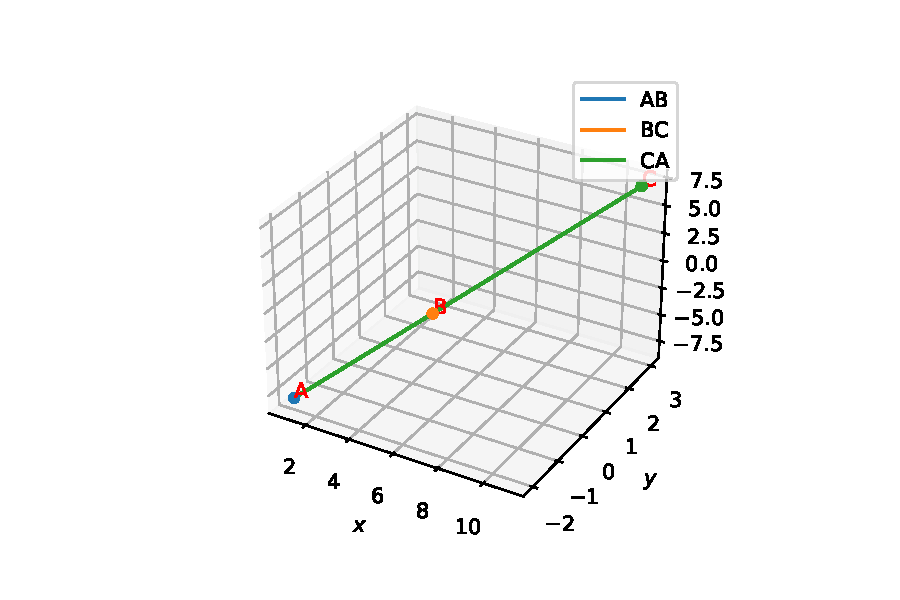
\includegraphics[width=\columnwidth]{A1_figure.pdf}
	\caption{The given points are collinear}
	\label{}
\end{figure}
\end{enumerate}
\end{document}
